\section{Rectificatifs du rapport de spécifications fonctionnelles}
\label{sec:rect}

Cette section a pour but d'énoncer et de justifier les différences constatées entre les fonctionnalités prévues dans le rapport de spécifications fonctionnelles~\cite{spec_fonc} et leur implémentation lors de la phase de développement. La {\sc sous-section}~\ref{subsec:archi} commence d'abord par énoncer les modifications les plus générales concernant l'architecture du logiciel, avant d'entrer plus en profondeur dans le code dans les sous-sections suivantes.

\subsection{Architecture générale}
\label{subsec:archi}

La {\sc Figure} \ref{fig:archiPrevue} illustre l'architecture générale imaginée lors du rapport de spécifications fonctionnelles~\cite{spec_fonc}. Suite à des contraintes techniques, notamment dûes au fait qu'un programme Java (ADTool dans notre cas) est difficilement contrôlable depuis un programme C\#, l'architecture a été revue pour correspondre à celle présentée à la {\sc Figure}~\ref{fig:archiReelle}. C'est pourquoi ADTool ne fait finalement pas partie intégrante de Glasir, mais est lancé en tant que simple \og viewer \fg{} d'ADTrees. En effet, il est impossible, depuis Glasir, de détecter des modifications faites dans ADTool, comme par exemple la modification d'une valuation de l'une des feuilles de l'ADTree. Par conséquent, la décision fut prise de désactiver toutes les fonctions d'édition dans ADTool lorsque Glasir se lance, donnant ainsi à ADTool un mode spécial baptisé \og viewmode \fg{}. Dans ce mode, l'utilisateur ne peut que visualiser un ADTree, sans pouvoir le modifier (les menus et les raccourcis clavier ont été supprimés). De plus, la bibliothèque de modèles n'est plus incluse dans Glasir : cette décision est justifiée dans la {\sc sous-section}~\ref{ssec:bib}.

		\begin{figure}[H]
            \centering
                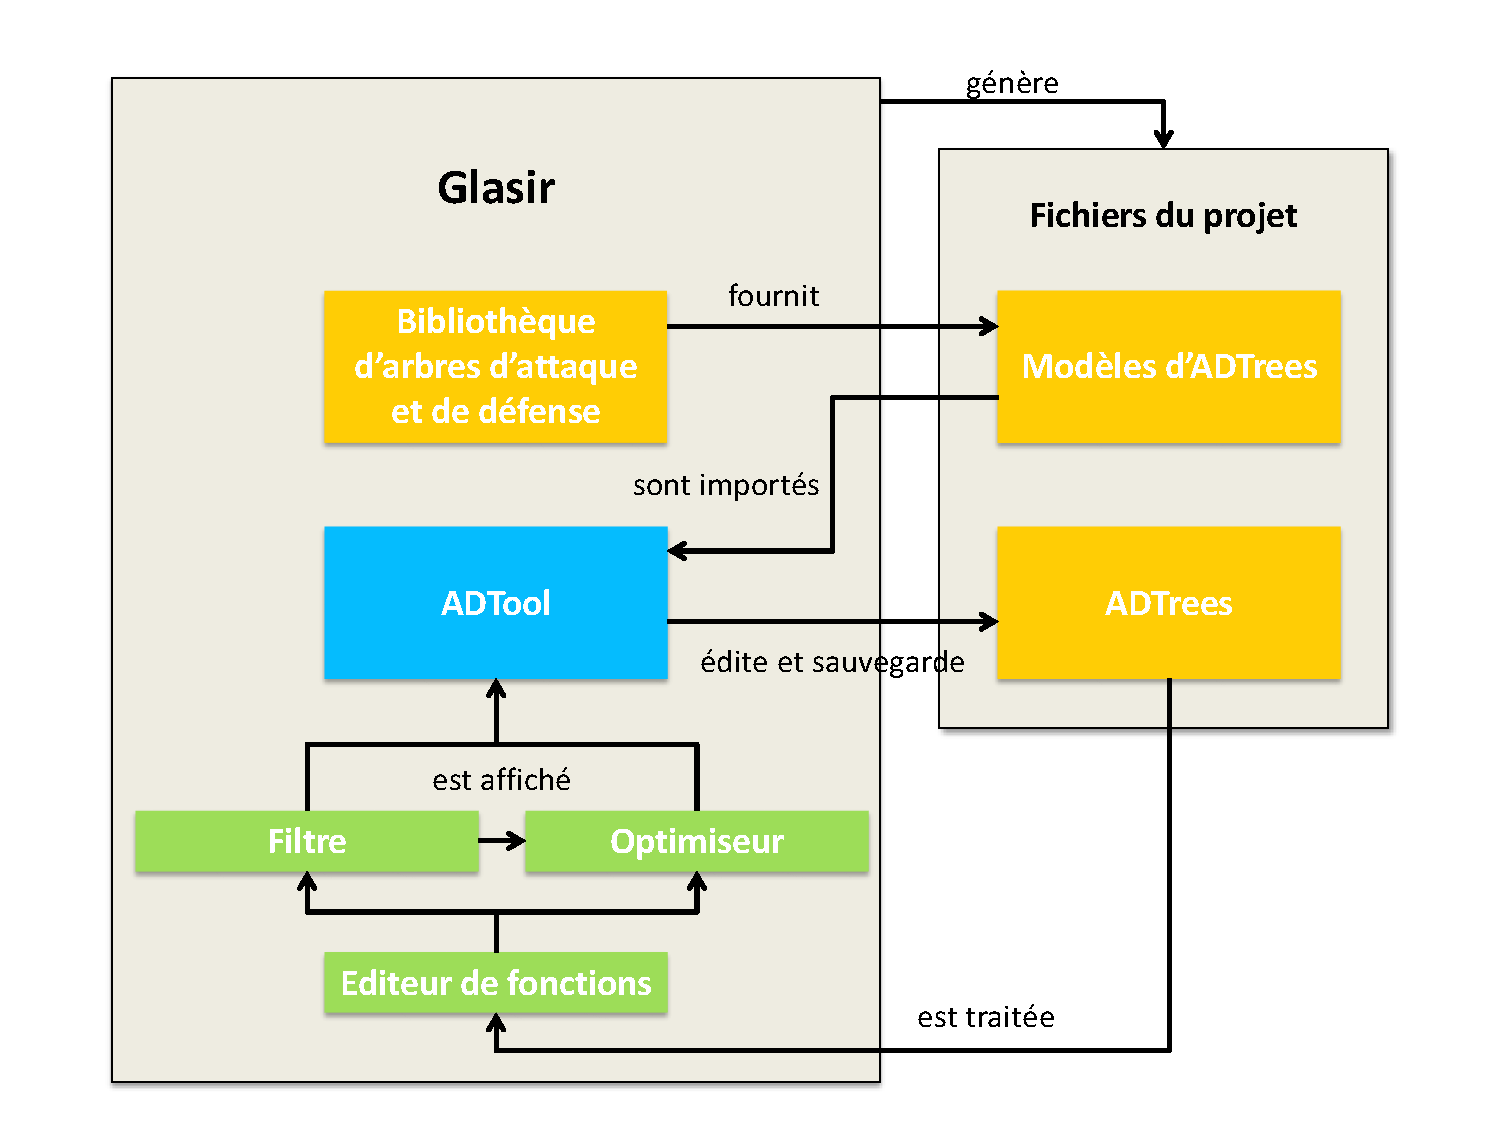
\includegraphics[width=0.8\textwidth]{figure/archiGlasir.pdf}
            \caption{Architecture initialement prévue.}
            \label{fig:archiPrevue}
        \end{figure}
	
        
        \begin{figure}[H]
            \centering
                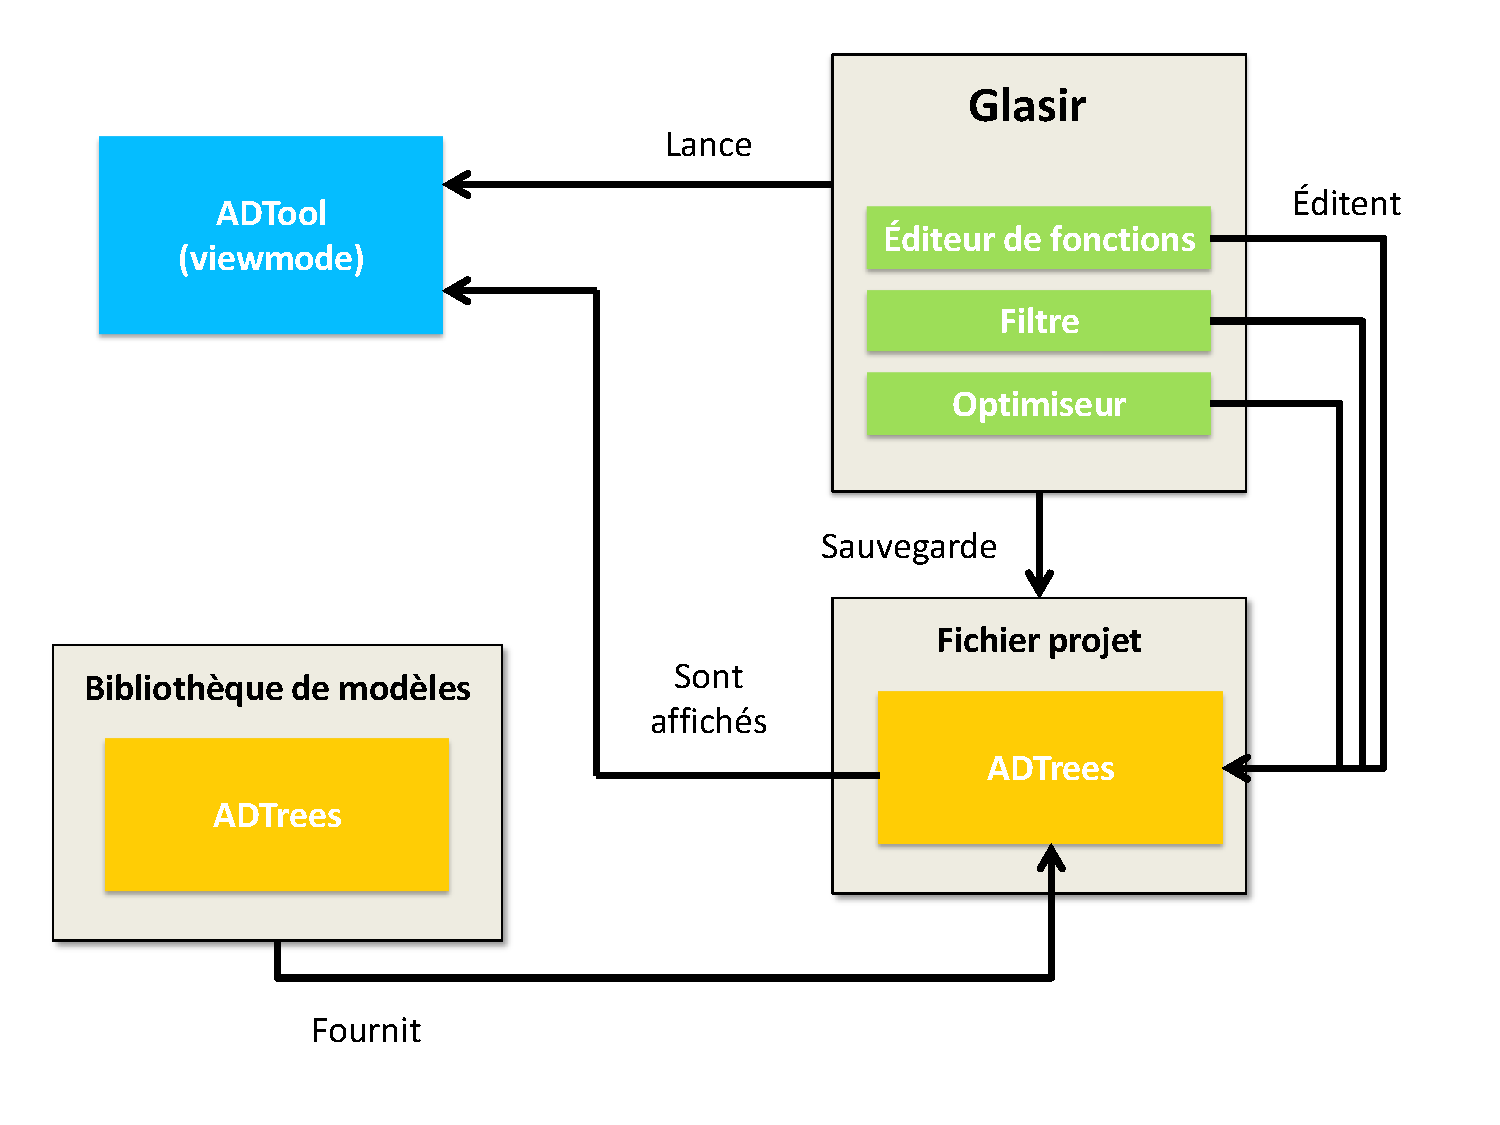
\includegraphics[width=0.8\textwidth]{figure/archiReelle.pdf}
            \caption{Architecture réelle.}
            \label{fig:archiReelle}
        \end{figure}
        
Les modules principaux de Glasir que sont l'Éditeur de fonctions, le Filtre et l'Optimiseur ont eux aussi été un peu revus par rapport à l'implémentation prévue dans le rapport de conception~\cite{conception}. Ces changements sont principalement liés à des questions de cohérence soulevées après le début du développement. Les {\sc sous-sections}~\ref{ssec:editeurFct},~\ref{ssec:implemFiltre} et~\ref{ssec:algoOptim} détaillent les modifications apportées à ces modules.

\subsection{Algorithme de l'Éditeur de fonctions}
\label{ssec:editeurFct}

Bien que nous n'ayons pas jugé nécessaire de détailler l'algorithme de l'Éditeur de fonctions lors de la rédaction du rapport de spécifications fonctionnelles~\cite{spec_fonc}, celui-ci s'est révélé plus délicat à implémenter que prévu. Son nouveau fonctionnement est donc détaillé ci-après, par une présentation de l'{\sc algorithme}~\ref{algo:functionEdition} qui a été effectivement implémenté.

	\begin{algorithm}[H]
            \caption{functionEdition(racine, param1, param2, function)}
            \label{algo:functionEdition}
            \begin{algorithmic}
		\IF{type(racine) == defense}
			\FORALL{sub \textbf{in} fils(racine)}
				\STATE functionEdition(sub, param1, param2, function)
			\ENDFOR
			\RETURN
		\ENDIF
		\STATE
		\IF{type(racine) == feuille}
			\STATE p1 = param1(racine)
			\STATE p2 = param2(racine)
			\STATE newParam(racine) = function(p1,p2)
			\RETURN
		\ELSE
			\FORALL{sub \textbf{in} fils(racine)}
				\IF {(type(sub) == defense}
					\STATE p1 = param1(racine)
					\STATE p2 = param2(racine)
					\STATE newParam(racine) = function(p1,p2)
				\ENDIF
				\STATE functionEdition(sub, param1, param2, function)
			\ENDFOR
		\ENDIF
            \end{algorithmic}
        \end{algorithm}

 Les notations non explicites de l'{\sc algorithme}~\ref{algo:functionEdition} sont présentées ci-dessous :
        \begin{itemize}
            \item \verb|racine| correspond au nœud racine de l'arbre ou sous-arbre manipulé ;
            \item \verb|param1| est une fonction renvoyant la valeur du 1\ier{} paramètre qui nous intéresse pour un nœud donné ;
            \item \verb|param2| est une fonction renvoyant la valeur du 2\ieme{} paramètre qui nous intéresse pour un nœud donné ;
            \item \verb|function| est une fonction calculant un résultat à partir de deux paramètres ;
            \item \verb|fils| est une fonction renvoyant la liste des fils du nœud passé en paramètre ;
            \item \verb|mode| précise si il s'agit d'un nœud disjonctif ou conjonctif ;
            \item \verb|type| précise si il s'agit d'un nœud d'attaque ou de défense, ou bien d'une feuille.
        \end{itemize}

    L'algorithme de l'Éditeur de fonctions est donc un algorithme récursif, qui cherche les feuilles de l'ADTree pour ajouter le nouveau paramètre à celles-ci. 

\subsection{Algorithme du Filtre}
\label{ssec:implemFiltre}

L'algorithme original du Filtre, représenté par l'{\sc algorithme}~\ref{algo:filtre}, comportait quelques erreurs telles que la possibilité de conserver des sous-n\oe{}uds d'un n\oe{}ud conjonctif qui ne respectaient pas la condition de filtrage. Cet algorithme a donc été corrigé en conséquence pour devenir l'{\sc algorithme}~\ref{algo:filtreReel} qui a été implémenté.

 	\begin{algorithm}[H]
            \caption{filtre(racine, rules)}
            \label{algo:filtre}
            \begin{algorithmic}
                \FOR{r in rules}
                    \IF{not r(racine)}
                        \STATE delete(r) // will delete subtrees as well
                        \RETURN
                    \ENDIF
                \ENDFOR
                \STATE
                \FOR{n in fils(racine)}
                    \STATE filtre(n, rules)
                \ENDFOR
            \end{algorithmic}
        \end{algorithm}
        

 	\begin{algorithm}[H]
            \caption{filtre(racine, param, valLim)}
            \label{algo:filtreReel}
            \begin{algorithmic}
	\STATE val = param(racine)
	\STATE
	\IF {pire(val, valLim)}
		\STATE delete(racine) // will delete subtrees as well
		\RETURN
	\STATE
	\ELSE
		\IF{mode(racine) == et}
			\FORALL{sub \textbf{in} fils(racine)}
				\STATE subval = sub.param
				\STATE filtre(sub, param, valLim+subval-val)
			\ENDFOR
		\ELSE
			\FORALL{sub \textbf{in} fils(racine)}
				\STATE filtre(sub, param, valLim)
			\ENDFOR
		\ENDIF
	\ENDIF
            \end{algorithmic}
        \end{algorithm}

    Dans l'{\sc algorithme}~\ref{algo:filtreReel}, \verb|valLim| est la valeur limite (maximale ou minimale selon les cas) acceptée pour le paramètre \verb|param| avec lequel on souhaite filtrer l'ADTree. Et \verb|pire| est une fonction renvoyant \emph{vrai} si son 1\ier{} paramètre \verb|val| est moins bon (c'est-à-dire inférieur ou supérieur, selon les cas) que son 2\ieme{} paramètre \verb|valLim| pour le domaine de valuation considéré. Elle renvoie \emph{faux} dans le cas contraire.

\subsection{Algorithme de l'Optimiseur}
\label{ssec:algoOptim}

    L'algorithme initial de l'Optimiseur, tel que décrit dans le rapport de spécifications fonctionnelles~\cite{spec_fonc}, est rappelé par l'{\sc algorithme}~\ref{algo:opti}.

         \begin{algorithm}[H]
            \caption{opti(racine, param)}
            \label{algo:opti}
            \begin{algorithmic}
                \STATE l\_fils = fils(racine)
                \IF{vide(l\_fils)}
                    \RETURN
                \ENDIF
                \STATE
                \IF{mode(racine) == ou}
                    \STATE v = param(racine)

                    \FOR{n in l\_fils}
                        \IF{not defense(n) and param(n) != v}
                            \STATE delete(n) // will delete subtrees as well
                        \ENDIF
                    \ENDFOR
                \ENDIF
                \STATE
                \FOR{n in fils(racine)}
                    \STATE opti(n, param)
                \ENDFOR
            \end{algorithmic}
        \end{algorithm}

Après avoir implémenté le Filtre, il est apparu qu'il était possible de l'utiliser pour simplifier l'implémentation de l'Optimiseur. Le nouvel algorithme obtenu (l'{\sc algorithme}~\ref{algo:optiReel}) n'impactant pas le résultat, c'est finalement lui qui a été choisi pour coder l'Optimiseur.

	\begin{algorithm}[H]
            \caption{opti(racine, param)}
            \label{algo:optiReel}
            \begin{algorithmic}
		\STATE v = param(racine)
		\STATE filtre(racine, param, v)
            \end{algorithmic}
        \end{algorithm}

    La présente section a permis de décrire les différences constatées à la fin du projet entre les promesses du rapport de spécifications fonctionnelles~\cite{spec_fonc} et l'implémentation réelle. Un autre rapport avait été rédigé avant le début du développement, celui de conception~\cite{conception}. Là encore, des écarts sont constatés avec ce qui a été codé, c'est ce dont fait état la {\sc section}~\ref{sec:rectConc}. 

\newpage
\section{Rectificatifs du rapport de conception}
\label{sec:rectConc}
    
    Cette section a pour objectif de comparer les fonctionnalités décrites lors du rapport de conception~\cite{conception} à celles qui ont été ensuite implémentées.

	\subsection{Affichage multiple des paramètres}

    Cette nouveauté n'a finalement pas été mise en place. En effet, l'étude approfondie du code source d'ADTool a montré qu'un tel changement aurait nécessité une refonte quasi-totale de la structure du logiciel. De telles modifications auraient demandé un temps de travail bien trop conséquent comparé au temps disponible pour la réalisation du projet. De toute manière, l'intérêt de ce nouvel affichage avait finalement été remis en cause : le risque de perdre en clarté et en lisibilité lors de la manipulation des ADTrees avait semblé trop important.

	\subsection{Couper/copier/coller}

	La {\sc Figure} \ref{fig:copypastePrevu} rappelle la fonctionnalité de couper/copier/coller telle qu'imaginée lors du rapport de conception~\cite{conception}. Après avoir mieux pris connaissance de la structure interne d'ADTool, il a paru beaucoup plus simple de réaliser cette fonctionnalité comme illustré sur la {\sc Figure} \ref{fig:copypasteReel}.
	
	
		\begin{figure}[H]
            \centering
                
\includegraphics[width=0.8\textwidth]{figure/copiercoller.png}
            \caption{Diagramme de classes prévu pour le couper/copier/coller.}
            \label{fig:copypastePrevu}
        \end{figure}
        
        \begin{figure}[H]
            \centering
                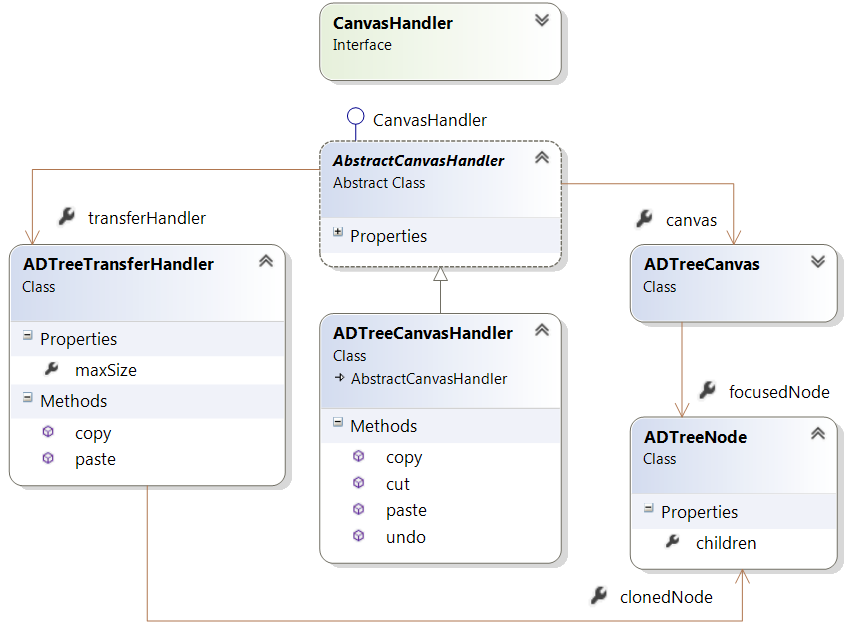
\includegraphics[width=0.9\textwidth]{figure/copiercollerReel.png}
            \caption{Diagramme de classes réellement implémenté pour le couper/copier/coller.}
            \label{fig:copypasteReel}
        \end{figure}

        Dans ADTool, un ADTree est en réalité un \emph{ADTreeNode} possédant des fils, qui sont eux-mêmes des \emph{ADTreeNode}. L'ADTree courant est affiché à l'écran via un \emph{ADTreeCanvas}. Les actions au clavier et à la souris réalisées par l'utilisateur sont captées par la classe \emph{AbstractCanvasHandler}, qui possède le \emph{ADTreeCanvas} sur lequel agit l'utilisateur. Il a donc été ajouté à l'\emph{AbstractCanvasHandler} un attribut de \emph{ADTreeTransferHandler}, une nouvelle classe qui contient les méthodes de copie et de collage d'un \emph{ADTreeNode}. Ainsi, lorsque l'utilisateur lance la commande \og couper \fg{}, par exemple, cette dernière est captée par la classe \emph{CanvasHandler} qui demande alors à sa classe parente (\emph{AbstractCanvasHandler}) de récupérer l'\emph{ADTreeNode} à couper (il s'agit de l'attribut \emph{focusedNode} de \emph{ADTreeCanvas}). L'\emph{ADTreeTransferHandler} se charge ensuite de l'opération de copie en stockant dans \emph{clonedNode} un clone de l'\emph{ADTreeNode} coupé. Dans le cas de l'action \og couper \fg{}, la suppression de l'ADTree coupé est gérée en interne par l'\emph{AbstractCanvasHandler}. Pour le collage, les opérations sont sensiblement identiques, sauf que le clone stocké par l'\emph{ADTreeTransferHandler} est restitué à l'\emph{AbstractCanvasHandler} qui se charge de l'ajouter à son \emph{ADTreeCanvas}.
       
	\subsection{Annulation des dernières actions}

		 La {\sc Figure}~\ref{fig:ctrlzPrevu} illustre l'implémentation de l'annulation de la dernière action telle qu'imaginée lors du rapport de conception~\cite{conception}, dans lequel il n'était pas prévu de pouvoir effectuer plusieurs annulations à la suite. De la même façon que pour le couper/copier/coller, la structure d'ADTool a conduit à implémenter l'annulation différemment, comme indiqué sur la {\sc Figure}~\ref{fig:ctrlzReel}. 
		 
        \begin{figure}[H]
            \centering
                
\includegraphics[width=0.8\textwidth]{figure/ctrlz.png}
            \caption{Diagramme de classes prévu pour l'annulation des dernières actions.}
            \label{fig:ctrlzPrevu}
        \end{figure}
        
        \begin{figure}[H]
            \centering
                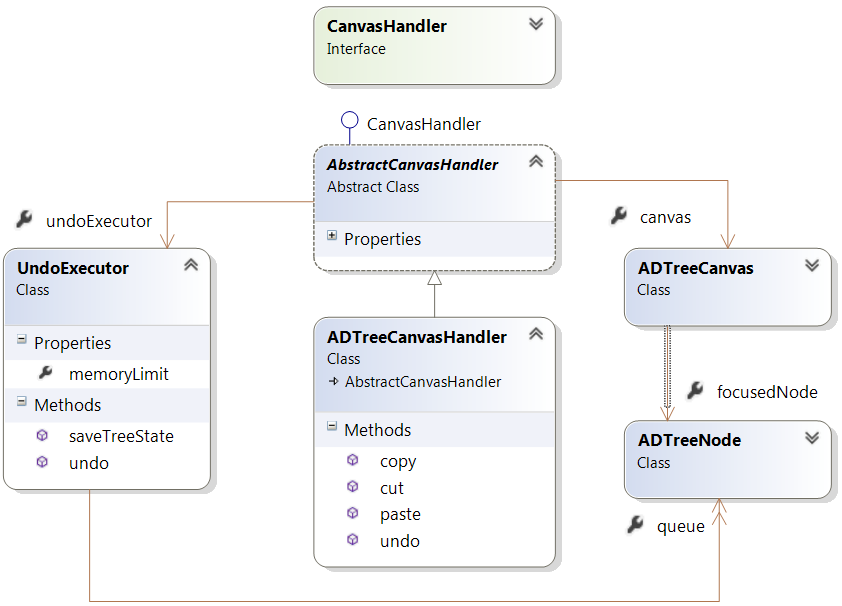
\includegraphics[width=0.8\textwidth]{figure/ctrlzReel.png}
            \caption{Diagramme de classes réellement implémenté pour l'annulation des dernières actions.}
            \label{fig:ctrlzReel}
        \end{figure}

        En effet, associer chaque action à une classe se révélait trop fastidieux, étant donné le grand nombre d'actions possibles. L'\emph{AbstractCanvasHandler} se voit donc doté d'un attribut de \emph{UndoExecutor}, une nouvelle classe qui contient les méthodes d'annulation. Lorsque l'utilisateur réalise une action, un clone de l'ADTree courant est stocké dans la pile de l'\emph{UndoExecutor}. Les clones sont dépilés et rechargés dans l'\emph{ADTreeCanvas} lorsque l'utilisateur utilise la fonctionnalité d'annulation. Afin d'éviter une saturation de la mémoire, la pile ne peut contenir qu'un certain nombre de clones de l'ADTree, supprimant si besoin le plus ancien pour pouvoir ajouter le plus récent. Il est à noter que plus l'ADTree est petit, plus le nombre d'actions annulables est grand, car la pile peut contenir plus de clones avant d'arriver à saturation. Dans le pire des cas, si l'ADTree est conséquent (dans notre cas, s'il contient plus de 1000 n\oe{}uds), seule la dernière action sera annulable. 

	\subsection{Bibliothèque de modèles}
    \label{ssec:bib}
		La {\sc Figure} \ref{fig:library} illustre l'implémentation de la bibliothèque de modèles telle qu'imaginée lors du rapport de conception~\cite{conception}. 
		
		\begin{figure}[H]
            \centering
                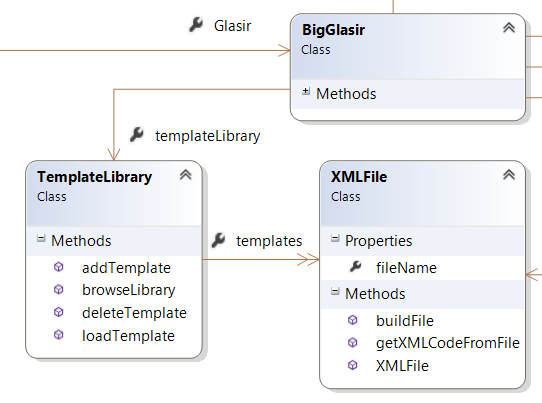
\includegraphics[width=0.75\textwidth]{figure/library.png}
            \caption{Diagramme de classes prévu pour la bibliothèque de modèles.}
            \label{fig:library}
        \end{figure}

        Finalement, cette bibliothèque se présente comme un simple dossier (fourni avec Glasir) contenant les modèles d'ADTrees. Ceux-ci portent sur le thème des transports en commun, ce qui correspond à l'étude de cas dans le cadre de ce projet mais ne doit pas restreindre l'utilisation de Glasir. C'est pourquoi il a été décidé de la fournir séparée du logiciel, pour que ce dernier reste adapté à l'analyse en sécurité de n'importe quel système.